\documentclass[16pt,aspectratio=169]{beamer}

\usetheme{metropolis}
\definecolor{Purple}{HTML}{911146}
\definecolor{Orange}{HTML}{CF4A30}
\setbeamercolor{alerted text}{fg=Orange}
\setbeamercolor{frametitle}{bg=Purple}
\usefonttheme{serif}
% \setsansfont{Liberation Sans}
% \setmonofont{Liberation Mono}

\usepackage{appendixnumberbeamer}

\usepackage{booktabs}
\usepackage[scale=2]{ccicons}

\usepackage{pgfplots}
\usepgfplotslibrary{dateplot}

\usepackage{xspace}
\newcommand{\themename}{\textbf{\textsc{metropolis}}\xspace}

% \usepackage{minted}
% \usemintedstyle{borland}

\usepackage{xeCJK}
\setCJKmainfont{Noto Serif CJK TC}

% \usecolortheme[snowy]{owl}


\title{Fine-Tuning can Distort Pretrained Features and Underperform Out-of-Distribution}
\subtitle{
    \textbf{Ananya Kumar, Aditi Raghunathan, Robbie Jones, Tengyu Ma, Percy Liang}\\
    Stanford University, Computer Science Department\\
    ICLR 2022 (Oral)
}
\date{\today}
\author{Hao-Ting Li (李皓庭)}
\institute{}

\makeatletter
\setbeamertemplate{title page}{
  \begin{minipage}[b][\paperheight]{\textwidth}
    \centering  % <-- Center here
    \ifx\inserttitlegraphic\@empty\else\usebeamertemplate*{title graphic}\fi
    \vfill%
    \ifx\inserttitle\@empty\else\usebeamertemplate*{title}\fi
    \ifx\insertsubtitle\@empty\else\usebeamertemplate*{subtitle}\fi
    \usebeamertemplate*{title separator}
    \ifx\beamer@shortauthor\@empty\else\usebeamertemplate*{author}\fi
    \ifx\insertdate\@empty\else\usebeamertemplate*{date}\fi
    \ifx\insertinstitute\@empty\else\usebeamertemplate*{institute}\fi
    \vfill
    \vspace*{1mm}
  \end{minipage}
}

\setbeamertemplate{title}{
%  \raggedright%  % <-- Comment here
  \linespread{1.0}%
  \inserttitle%
  \par%
  \vspace*{0.5em}
}
\setbeamertemplate{subtitle}{
%  \raggedright%  % <-- Comment here
  \insertsubtitle%
  \par%
  \vspace*{0.5em}
}
\makeatother


\begin{document}
\metroset{titleformat frame=smallcaps}

\maketitle

\begin{frame}
    \frametitle{Introduction}

    Pretraining a model on a large dataset before transferring to a downstream task's training data substantially improves accuracy over training from scratch—for example, pretraining a ResNet-50 on unlabeled ImageNet boosts accuracy on CIFAR-10 from 94\% to 98\% (Chen et al., 2020a;b)

    Two transfer methods:
    \begin{itemize}
        \item fine-tuning: running gradient descent on all the model parameters
        \item linear probing: tuning the head but freezing lower layers
    \end{itemize}

    Fine-tuning can do worse than linear probing in the presence of a large distribution shift.
\end{frame}

\begin{frame}
    \frametitle{Fine-tuning vs. Linear Probing vs. LP-FT (1/2)}

    \begin{figure}[htbp]
        \centering
        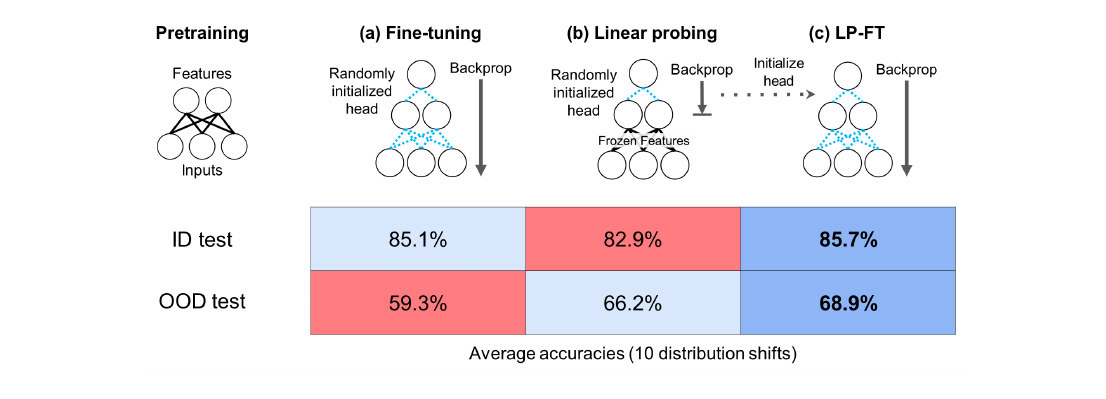
\includegraphics[width=\textwidth]{figures/illustration.png}
        \caption{Given a good feature extractor (top-left), a randomly initialized head is added to map features to outputs.}
    \end{figure}

\end{frame}

\begin{frame}
    \frametitle{Fine-tuning vs. Linear Probing vs. LP-FT (2/2)}

    \begin{figure}[htbp]
        \centering
        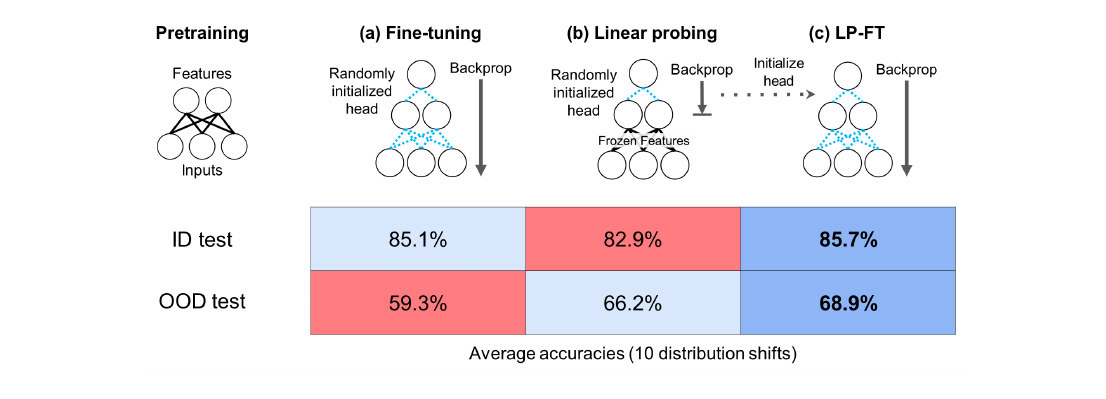
\includegraphics[width=\textwidth]{figures/illustration.png}
    \end{figure}

    Our theory indicates that fine-tuning can distort the pretrained feature extractor and lead to poor OOD accuracy, but {\color{blue} initializing with a linear probed head} can fix this—empirically LP-FT gets better accuracies both ID and OOD.

\end{frame}

\section{Why Fine-Tuning Can Underperform OOD}

\begin{frame}
    \frametitle{Setup: Task and Evaluation (1/2)}

    Given training examples sampled from some distribution $P_{\text {id}}$, our goal is to learn a predictor $f: \mathbb{R}^d \rightarrow \mathcal{Y}$ to map inputs $x \in \mathbb{R}^d$ to outputs $y \in \mathcal{Y}$.

    We evaluate predictors on their standard ``in-distribution'' (ID) performance $L_{\mathtt{id}}$ on new test samples drawn from $P_{\mathtt {id}}$ that the training data is also sampled from.

    We also evaluate classifiers on their ``out-of-distribution'' (OOD) performance $L_{\mathtt {ood}}$ on test samples drawn from a new distribution $P_{\mathtt {ood}}$ that is different from $P_{\mathtt {id}}$.

    Formally, for some loss function $\ell$, we evaluate classifiers on:

    \begin{equation}
        L_{\mathtt{id}}(f)=\underset{(x, y) \sim P_{\mathtt{id}}}{\mathbb{E}}[\ell(f(x), y)] \text { and } L_{\mathtt{ood}}(f)=\underset{(x, y) \sim P_{\mathtt{ood}}}{\mathbb{E}}[\ell(f(x), y)]
    \end{equation}

\end{frame}

\begin{frame}
    \frametitle{Setup: Models (2/2)}

    In this work, we focus on predictors that leverage pretrained representations. 

    We parameterize the final predictor $f$ as follows: given features $g_B(x) \in \mathbb{R}^k$ for some feature extractor parameters $B \in \mathcal{B}$, and a linear ``head'' $v \in \mathcal{V}$, we have $f_{v, B}(x)=v^{\top} g_B(x)$. 
    \begin{itemize}
        \item $f$: final predictor
        \item $g_B(x) \in \mathbb{R}^k$: features
        \item $B \in \mathcal{B}$: feature extractor parameters
        \item $v \in \mathcal{V}$: linear head
    \end{itemize}

    In our experiments (Section 4), $g_B$ is a deep network and in our theory (Section 3), $g_B$ is a linear projection.

\end{frame}

\begin{frame}
    \frametitle{Linear Over-Parameterized Setting: Models (1/7)}
    
    For our analysis, we focus on regression, where $\mathcal{Y}=\mathbb{R}$ and $\ell(\hat{y}, y) = (\hat{y}-y)^2$ is the squared loss.

    In this section, we study models where the feature extractor is linear, i.e. $f_{v,B}(x) = v^\top Bx$ where $B \in \mathcal{B}=\mathbb{R}^{k \times d}$, and $v \in \mathcal{V} = \mathbb{R}^k$.
\end{frame}

\begin{frame}
    \frametitle{Linear Over-Parameterized Setting: Good Pretrained Features (2/7)}

    For simplicity, we assume the models are well-specified i.e. $y=v_{\star}^{\top} B_{\star} x$ where $v_{\star} \in \mathbb{R}^k$ and $B_{\star} \in \mathbb{R}^{k \times d}$.

    Note that $B_{\star}$ and $v_{\star}$ are only unique up to rotations, i.e., for any rotation matrix $U,\left(U v_{\star}\right)^\top \left(U B_{\star}\right) x=v_{\star}^\top  B_{\star} x$.\footnote{The inverse of a rotation matrix is its transpose: $U^\top U = I$.}

    As in prior work (Tripuraneni et al., 2020) suppose $B_{\star}$ and $B_0$ have been orthogonalized to have orthonormal rows. We have a pretrained feature extractor $B_0$ close to $B_{\star}$, so $d(B_0, B_{\star}) < \epsilon$ where the distance $d$ is defined as:
    \begin{equation}
        d(B, B^\prime) = \min_{U} \| B-UB^\prime \|_2
    \end{equation}

\end{frame}

\begin{frame}
    \frametitle{Linear Over-Parameterized Setting: Training Data (3/7)}

    \begin{itemize}
        \item Let $X \in \mathbb{R}^{n \times d}, X \neq 0$ be a matrix encoding $n$ training examples from $P_{\mathtt {id}}$ where each of the $n$ rows is a training input. 
        \item Let $Y \in \mathbb{R}^n$ be the corresponding outputs. 
        \item Let $S=\operatorname{rowspace}(X)$ be the $m$-dimensional subspace spanning the training examples.
        \item We consider an over-parameterized\footnote{A model having more parameters than can be estimated from the data.} setting where $1 \leq m<d-k$. Intuitively, the input dimension $d$ is high (e.g., 10K), feature dimension $k$ is lower (e.g., 100) and $m$ is in the middle (e.g., 5K).
    \end{itemize}

\end{frame}

\begin{frame}
    \frametitle{Linear Over-Parameterized Setting: Large OOD Shift (4/7)}

    We assume that the OOD data contains examples outside the span of the training data.

    Formally, let $P_{\mathtt {ood}}$ have second moment $\Sigma=\mathbb{E}\left[x x^{\top}\right]$ where $x \sim P_{\mathtt {ood}}$, for invertible $\Sigma$.

\end{frame}

\begin{frame}
    \frametitle{Linear Over-Parameterized Setting: Training Methods (5/7)}

    Given training data and a pretrained feature extractor $B_0$, we study the two popular methods of linear probing (LP) and fine-tuning (FT) to learn the final predictor.

    Both methods involve optimizing the training loss via gradient descent (or variants).

    In order to effectively analyze these gradient based algorithms, we study vanishing step sizes leading to gradient flows.

    Gradient flows can be thought of as a continuous time analogue of gradient based methods and have been extensively studied in recent years as a way to understand gradient based methods (Gunasekar et al., 2017; Arora et al., 2018; Du et al., 2018).

\end{frame}

\begin{frame}
    \frametitle{Linear Over-Parameterized Setting: Training Loss \& Gradient Flow (6/7)}

    
    Formally, for training loss $\widehat{L}(v, B) = \| XB^\top v - Y \|_2^2$ , the gradient flow differential equations for LP and FT are as follows:

    \begin{equation}
        \partial_t v_{\mathtt{ft}}(t)=-\nabla_v \widehat{L}\left(v_{\mathtt{ft}}(t), B_{\mathtt{ft}}(t)\right),
        \partial_t B_{\mathtt{ft}}(t)=-\nabla_B \widehat{L}\left(v_{\mathtt{ft}}(t), B_{\mathtt{ft}}(t)\right)
    \end{equation}

    \begin{equation}
        \partial_t v_{\mathtt{lp}}(t)=-\nabla_v \widehat{L}\left(v_{\mathtt{lp}}(t), B_0\right), \partial_t B_{\mathtt{lp}}(t)=0,
    \end{equation}

    initialized with $B_{\mathtt{ft}}(0)=B_{\mathtt{lp}}(0)=B_0$ and $v_{\mathtt{ft}}(0)=v_{\mathtt{lp}}(0)=v_0$. 

    \begin{itemize}
        \item In practice, the head parameter $v_0$ is initialized randomly —our results hold for any standard random initialization (Glorot \& Bengio), for example $v_0 \sim \mathcal{N}\left(0, \sigma^2 I\right)$ for any $\sigma^2$, or zero initialization where $v_0=0$. 
    \end{itemize}

    Recall that the initial value of the feature extractor $B_0$ is obtained via pretraining.

\end{frame}

\begin{frame}
    \frametitle{Linear Over-Parameterized Setting: Training Loss \& Gradient Flow (7/7)}

    The final LP and FT solutions are the limit points of the corresponding gradient flows:

    \begin{equation}
        \begin{aligned}
            & v_{\mathtt{ft}}^{\infty}=\lim _{t \rightarrow \infty} v_{\mathtt{ft}}(t) \text { and } B_{\mathtt{ft}}^{\infty}=\lim _{t \rightarrow \infty} B_{\mathtt{ft}}(t), \\
            & v_{\mathtt{lp}}^{\infty}=\lim _{t \rightarrow \infty} v_{\mathtt{lp}}(t) \text { and } B_{\mathtt{lp}}^{\infty}=\lim _{t \rightarrow \infty} B_{\mathtt{lp}}(t)=B_0 .
        \end{aligned}            
    \end{equation}

\end{frame}

\begin{frame}
    \frametitle{Fine-Tuning Distorts Pretrained Features: Key Intuitions}

    Two observations to characterize when and why FT has higher OOD error than LP:

    \begin{itemize}
        \item Features get distorted: representations change only in the ID subspace (i.e., subspace spanned by the training data) and are unchanged in the orthogonal subspace.
        \item Distorted features can lead to higher OOD error.
    \end{itemize}
    
\end{frame}

\begin{frame}
    \frametitle{Feature Distortion}

    \begin{itemize}
        
        \item The training loss: $\widehat{L}(v, B) = \| XB^\top v - Y \|_2^2$
        \item The derivative of the training loss: $\nabla_B \widehat{L}(v, B) = 2v (Y-XB^\top v)^\top X$
        \item By definition, if $u$ is a direction orthogonal to the training subspace $S = \operatorname{rowspace}(X)$, then $\nabla_B \widehat{L}(v, B) u = 0$, that is the gradient updates to $B$ do not modify $Bu$ for $u \in S^\bot$.\footnote{$S^\perp$: 子空間 $S$ 的正交補餘 (orthogonal complement, perpendicular complement),表示與 $S$ 正交的所有向量的集合}
        \item However, the gradient is non-zero for directions $u$ in the ID subspace and the corresponding features $Bu$ change across the fine-tuning process.
        \item We call this feature distortion: the features in some directions are changed but not others. Next, we explain why this can lead to high OOD error.
    \end{itemize}

\end{frame}

\begin{frame}
    \frametitle{Distorted Features Can Lead to Higher OOD Error (1/5)}

    Consider a toy example where $d=2$ and the dimensionality of the representations $k=1$. The linear head $v$ is a scalar quantity that denotes how much the feature extractor $B$ has to be scaled by.

    \begin{figure}[htbp]
        \centering
        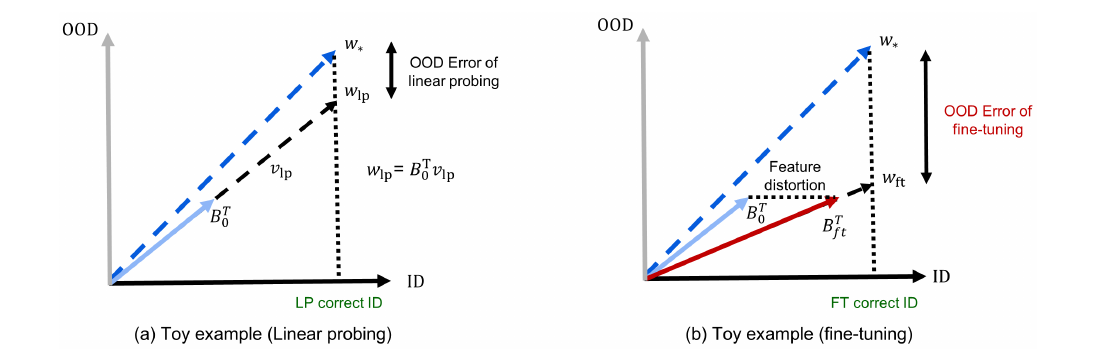
\includegraphics[width=.9\textwidth]{figures/toy-example.png}
        \caption{A toy version of our theory illustrating why fine-tuning distorts features, with inputs in 2D.}
    \end{figure}

\end{frame}

\begin{frame}
    \frametitle{Distorted Features Can Lead to Higher OOD Error (2/5)}

    \begin{figure}[htbp]
        \centering
        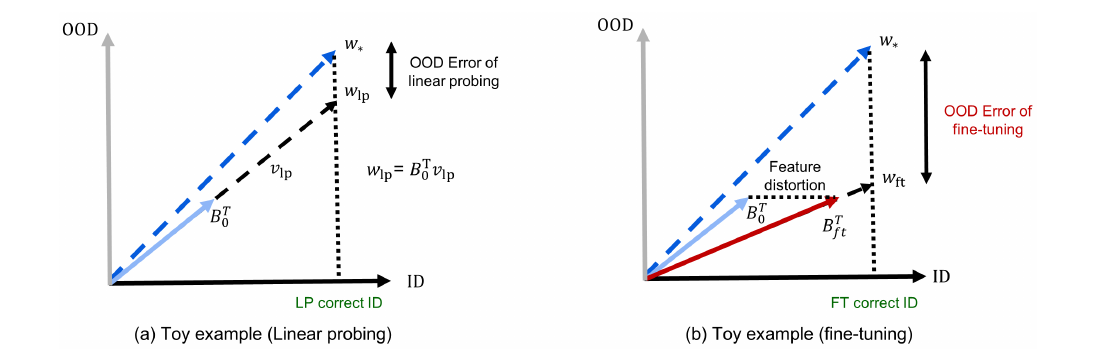
\includegraphics[width=\textwidth]{figures/toy-example.png}
    \end{figure}

    \begin{itemize}
        \item Both fine-tuned and linear probed estimators match the true parameter in the ID subspace (since $w_{\mathtt{lp}}$, $w_{\mathtt{ft}}$, $w_{\mathtt{\star}}$ have the same projection on the $x$-axis).
    \end{itemize}

\end{frame}

\begin{frame}
    \frametitle{Distorted Features Can Lead to Higher OOD Error (3/5)}
    \begin{figure}[htbp]
        \centering
        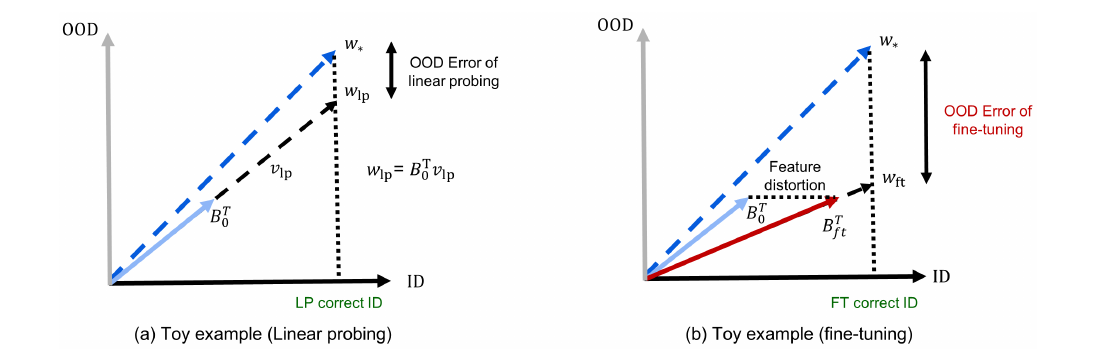
\includegraphics[width=\textwidth]{figures/toy-example.png}
    \end{figure}

    \begin{itemize}
        \item If the feature extractor were optimal or scaled versions of the optimal, good performance on the ID subspace would translate to good performance everywhere, even in directions orthogonal to the ID subspace.
    \end{itemize}

\end{frame}

\begin{frame}
    \frametitle{Distorted Features Can Lead to Higher OOD Error (4/5)}
    \begin{figure}[htbp]
        \centering
        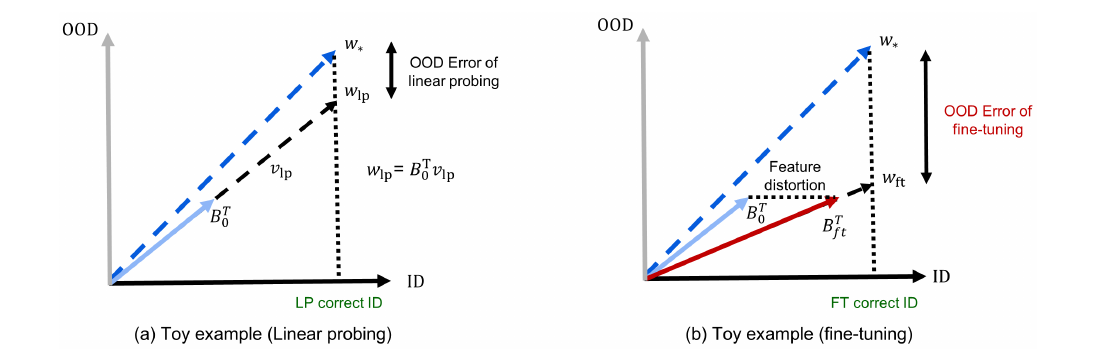
\includegraphics[width=\textwidth]{figures/toy-example.png}
    \end{figure}

    \begin{itemize}
        \item However, in FT, the features change only for inputs in the ID subspace and thus the updated features are not simply scaled but distorted.
        \item In this case even if the ID error is low, error in directions orthogonal to the ID subspace can be high, leading to high OOD error.
    \end{itemize}

\end{frame}

\begin{frame}
    \frametitle{Distorted Features Can Lead to Higher OOD Error (5/5)}

    \begin{itemize}
        \item The only way the pretrained features are not distorted and only scaled during FT is if the initial feature extractor $B_0$ is exactly aligned with the ID subspace.
        \item However, if the angle between $B_0$ and the x-axis is non-zero, the updates would lead to distortions.
        \item How to measure the alignment between $B_0$ and the ID subspace?
        \begin{itemize}
            \item[$\circ$] {\color{blue}Largest principal angle}
        \end{itemize}
    \end{itemize}

\end{frame}

\begin{frame}
    \frametitle{Definition 3.1: Largest Principal Angle}

    Let $A$ and $B$ be arbitrary subspaces, and $E$ and $F$ be matrices with orthonormal columns that span $A$ and $B$ respectively, with $r = \min(\operatorname{dim}(A), \operatorname{dim}(B))$. 
    
    Then $\cos \theta_{\mathtt{max}}(A, B) = \sigma_r (E^\top F)$, which is the $r$-th largest singular value of $E^\top F$.

\end{frame}

\begin{frame}
    \frametitle{Theorem 3.2}

    In the overparameterized linear setting, let $S^{\perp}= \operatorname{rowspace} (X)^{\perp}, R_0= \operatorname{rowspace} \left(B_0\right)$, and $v_{\star}, B_{\star}$ be the optimal parameters with $w_{\star}=B_{\star} v_{\star}$. 

    If $\cos \theta_{\mathtt{max}}\left(R_0, S^{\perp}\right)>0$, then for all time steps $t$, the OOD error of the fine-tuning iterates $\left(B_{\mathtt{ft}}(t), v_{\mathtt{ft}}(t)\right)$ is lower bounded:
    \begin{equation}
        \sqrt{L_{\mathtt{ood}}\left(v_{\mathtt{ft}}(t), B_{\mathtt{ft}}(t)\right)} \geq \sqrt{\sigma_{\mathtt{min}}(\Sigma)}\left(\frac{\cos \theta_{\mathtt{max}}\left(R_0, S^{\perp}\right)}{\sqrt{k}} \frac{\min \left(\varphi, \varphi^2 /\left\|w_{\star}\right\|_2\right)}{\left(1+\left\|w_{\star}\right\|_2\right)^2}-\epsilon\right),
    \end{equation}

    \begin{itemize}
        \item $\varphi^2=\left|\left(v_0^{\top} v_{\star}\right)^2-\left(v_{\star}^{\top} v_{\star}\right)^2\right|$ : initial head alignment error
        \item $\epsilon \geq d\left(B_0, B_{\star}\right)$ : the error in the pretrained feature extractor
    \end{itemize}

\end{frame}

\begin{frame}
    \frametitle{Proof Sketch (1/2)}

    \begin{enumerate}
        \item Since the features do not change for examples in $S^{\perp}$ (perpendicular to the training data), we show that in order to achieve low error on $S^{\perp}$ the linear head $v_{\mathtt{ft}}(t)$ would have to become very similar to the optimal $v_{\star}$ at some time $t$.
        \item The head initialization $v_0$ is random (or zero) and likely to be far from $v_{\star}$ (measured by the alignment error $\varphi$ ), so the head would have to change a lot to get close to $v_{\star}$.
    \end{enumerate}

\end{frame}

\begin{frame}
    \frametitle{Proof Sketch (2/2)}

    \begin{enumerate}
        \setcounter{enumi}{2}
        \item As we see from the fine-tuning gradient flow (3.2),$v_{\mathtt{ft}}(t)$ and $B_{\mathtt{ft}}(t)$ change in a ``coupled'' manner, and a ``balancedness'' invariant in Du et al. (2018) holds across the fine-tuning trajectory.
        \item Correspondingly, if $v_{\mathtt{ft}}(t)$ changes a lot and gets close to $v_{\star}$, the features $B_{\mathtt{ft}}(t)$ also change a lot for examples in $S$---we show that this would lead to high error on examples in $S$.
        \item Either way, fine-tuning would get some subspace ( $S$ or $S^{\perp}$ ) of examples wrong, leading to high OOD error.
    \end{enumerate}

\end{frame}

\begin{frame}
    \frametitle{Interpretations of Various Quantities}

    Theorem 3.2:

    $$
    \sqrt{L_{\mathtt{ood}}\left(v_{\mathtt{ft}}(t), B_{\mathtt{ft}}(t)\right)} \geq \sqrt{\sigma_{\mathtt{min}}(\Sigma)}\left(\frac{\cos \theta_{\mathtt{max}}\left(R_0, S^{\perp}\right)}{\sqrt{k}} \frac{\min \left(\varphi, \varphi^2 /\left\|w_{\star}\right\|_2\right)}{\left(1+\left\|w_{\star}\right\|_2\right)^2}-\epsilon\right),
    $$

    \begin{itemize}
        \item Quality of pretrained features $(\epsilon)$.
        \item Alignment error of random head initialization $\left(\varphi^2\right)$. 
    \end{itemize}

\end{frame}

\begin{frame}
    \frametitle{Interpretations of Various Quantities: Quality of Pretrained Features $(\epsilon)$}

    \begin{itemize}
        \item To unpack the bound consider a special case where the pretrained features are perfect $(\epsilon=0)$. 
        \item With perfect features, Proposition A.21 shows that linear probing gets zero OOD error. 
        \item Theorem 3.2 shows that $L_{\text {ood}}\left(v_{\mathtt{ft}}(t), B_{\mathtt{ft}}(t)\right)>0$ at all times $t$---so fine-tuning underperforms when the features are perfect.
    \end{itemize}

    Proposition A.21:
    
    In the overparameterized linear setting, let $R=\operatorname{rowspace}(B_0)$. If $B_0 = B_\star$, and $\cos \theta_{\mathtt{max}}(S, R) > 0$, then $L_{\mathtt{ood}}(v_{\mathtt{lp}}^\infty, B_0) = 0$ for all $t$.

\end{frame}

\begin{frame}
    \frametitle{Alignment Error of Random Head Initialization $\left(\varphi^2\right)$}

    \begin{itemize}
        \item The lower bound (Equation A.14) increases as $\varphi^2$ increases, because the gradient updates to the head and feature extractor are coupled. 
        \item If the head were somehow initialized perfectly at $v_{\star}$, fine-tuning updates may not increase the OOD error.
        \item However, when the head is randomly initialized as is\footnote{as is: 按原樣,表示某物的現有狀況,沒有任何修改或改進。} standard in fine-tuning, the alignment error is high, leading to high OOD error.
        \item We use this insight in Section 3.4 to show that better head initialization (via linear probing) improves OOD performance of fine-tuning.
    \end{itemize}

    Equation A.14:
    $$
    \sqrt{L_{\mathtt{ood}}\left(v_{\mathtt{ft}}(t), B_{\mathtt{ft}}(t)\right)} \geq \sqrt{\sigma_{\mathtt{min}}(\Sigma)}\left(\frac{\cos \theta_{\mathtt{max}}\left(R_0, S^{\perp}\right)}{\sqrt{k}} \frac{\min \left(\varphi, \varphi^2 /\left\|w_{\star}\right\|_2\right)}{\left(1+\left\|w_{\star}\right\|_2\right)^2}-\epsilon\right),
    $$

\end{frame}

\begin{frame}
    \frametitle{Linear Probing vs. Fine-tuning}

    We use our main theorem on fine-tuning (Theorem 3.2) and adapt prior work on linear probing to show that:
    
    Linear probing is better than fine-tuning OOD, but worse ID, when the ID distribution has density on a lower $m < d$ dimensional subspace $S$, and $B_0$ is close to $B_\star$.\footnote{$m$: subspace dimension; $d$: input dimension.}

\end{frame}

\begin{frame}
    \frametitle{Assumption 3.3: ID Subspace Assumption}

    We assume that the ID data lies on an $m$-dimensional subspace $S$ where $k<m<d-k$, and we have $n \geq m$ training examples.
 
    Formally, let $P_z$ be a distribution on $\mathbb{R}^m$ which has density, and let the columns of $F \in \mathbb{R}^{d \times m}$ form an orthonormal basis for $S$. Then $P_{\text {id}}$ has the distribution of $F z$ where $z \sim P_z$.

    Recall that the ID error is the expected mean-squared error over the ID distribution $P_{\text {id}}$:
    \begin{equation}
        L_{\text{id}}(v, B)=\underset{x \sim P_{\text {id}}}{\mathbb{E}}\left[\left(v_{\star}^{\top} B_{\star} x-v^{\top} B x\right)^2\right]
    \end{equation}

\end{frame}

\begin{frame}
    \frametitle{OOD Comparison}

    Under mild non-degeneracy conditions, we show that as the feature extractor error $\epsilon$ goes to $0$ , linear probing does much better than fine-tuning OOD: the ratio of the losses goes to $0$.

    The non-degeneracy conditions are similar to Section 3.2---we require that the training data cannot be exactly in the same direction or orthogonal to the pretrained features, formally that $\cos \theta_{\mathtt{max}}\left(R_*, S\right)$ and $\cos \theta_{\mathtt{max}}\left(R_*, S^{\perp}\right)$ are not $0$ where $R_*=\operatorname{rowspace}\left(B_{\star}\right)$.

\end{frame}

\begin{frame}
    \frametitle{Theorem 3.4 (Informal version of Theorem A.9)}

    In the linear overparameterized setting, under the ID subspace assumption (Assumption 3.3), if $\cos \theta_{\mathtt{max}}\left(R_*, S\right) \neq 0$ and $\cos \theta_{\mathtt{max}}\left(R_*, S^{\perp}\right) \neq 0$ where $R_*=\operatorname{rowspace}\left(B_{\star}\right)$, then,
    \begin{equation}
        \frac{L_{\mathtt{ood}}\left(v_{\mathtt{lp}}^{\infty}, B_0\right)}{L_{\mathtt{ood}}\left(v_{\mathtt{ft}}(t), B_{\mathtt{ft}}(t)\right)} \stackrel{p}{\rightarrow} 0 \text {, as } B_0 \rightarrow B_{\star} .
    \end{equation}

    \begin{itemize}
        \item This holds for all times $t$ for FT (and therefore also for the limit $v_{\mathtt{ft}}^{\infty}, B_{\mathtt{ft}}^{\infty}$ ) and the LP iterates converge to $v_{\mathtt{lp}}^{\infty}, B_0$ as a result of the gradient flow on a convex problem.
    \end{itemize}
    
    Intuitively, if the pretrained features are good, LP learns a near optimal linear head which has small OOD error (Lemma A.5) but fine-tuning has high OOD error (Theorem 3.2).

\end{frame}

\begin{frame}
    \frametitle{ID comparison}

    When the pretrained features have some error, we show that fine-tuning does better than linear probing ID because fine-tuning can update the features to fit the ID data.

\end{frame}

\begin{frame}
    \frametitle{Proposition 3.5}

    In the linear overparameterized setting, under the ID subspace assumption (Assumption 3.3), let $R_0=\operatorname{rowspace}\left(B_0\right)$, and $R_{\text {aug}}=\operatorname{Span}\left(\left\{w_{\star}\right\} \cup R_0\right)$. 

    Suppose $w_{\star} \notin R_0$, $\cos \theta_{\mathtt{max}}\left(S, R_{\mathtt{aug}}\right) \neq 0$, and that fine-tuning converges to a local minimum of its loss, then fine-tuning does better ID almost surely: $L_{\mathtt{id}}\left(v_{\mathtt{ft}}^{\infty}, B_{\mathtt{ft}}^{\infty}\right)<L_{\mathtt{id}}\left(v_{\mathtt{lp}}^{\infty}, B_0\right)$ with probability $1$ (over the randomness of the training examples).
    
    To summarize, we proved that there are tradeoffs between ID and OOD error: \\
    {\color{blue}FT has lower ID error but higher OOD error than LP.} 

\end{frame}

\begin{frame}
    \frametitle{A Simple Variant to Mitigate Tradeoffs: Linear Probing Then Fine-Tuning}

    The advantage of fine-tuning is it can adapt the feature extractor to fit the downstream task. 

    Can we keep this benefit while ensuring that our OOD error is low when we have good pretrained features?\\
    {\color{blue}Linear probing then fine-tuning.}

\end{frame}

\begin{frame}
    \frametitle{Why Linear Probing Then Fine-Tuning}

    Going back to Theorem 3.2, we see that the alignment error in the head initialization $\varphi^2=\left|\left(v_0^{\top} v_{\star}\right)^2-\left(v_{\star}^{\top} v_{\star}\right)^2\right|$ plays an important role. 
    
    The issue with FT was that under random or zero initialization, $\varphi^2$ is usually large and since the gradient updates to the feature extractor parameter are coupled with that of the head parameter, the features get distorted in a manner that increases the OOD error. 
    
    This suggests that {\color{blue}we should use a better head initialization}---one obtained from linear probing. 
    
    If the pretrained features are decent, a linear probed head would be much better aligned with $v_{\star}$ allowing the features to be updated in a manner that does not increase the OOD error much.

\end{frame}

\begin{frame}
    \frametitle{Proposition 3.6}

    Given perfect pretrained features $B_0=U B_{\star}$ for some rotation $U$. 
    Let $R_0= \operatorname{rowspace} \left(B_0\right)$. 
    Under the non-degeneracy conditions $\cos \theta_{\mathtt{max}}\left(R_0, S\right) \neq 0, \cos \theta_{\mathtt{max}}\left(R_0, S^{\perp}\right) \neq 0$:

    \begin{equation}
        \forall t, L_{\mathtt{ood}}\left(B_{\mathtt{ft}}(t)^{\top} v_{\mathtt{ft}}(t)\right)>0, \text { if } v_0 \sim \mathcal{N}\left(0, \sigma^2 I\right) \text { is randomly initialized (FT)},
    \end{equation}

    \begin{equation}
        \forall t, L_{\mathtt{ood}}\left(B_{\mathtt{ft}}(t)^{\top} v_{\mathtt{ft}}(t)\right)=0, \text { if } v_0 \text { is initialized to } v_{\mathtt{lp}}^{\infty} \text{(LP-FT)}.
    \end{equation}

\end{frame}

\section{Experiments}

\begin{frame}
    \frametitle{Distribution Shift Datasets}

    \begin{itemize}
        \item DomainNet (Peng et al., 2019; Tan et al., 2020)
        \item BREEDS-Living-17 (Santurkar et al., 2020)
        \item BREEDS-Entity-30 (Santurkar et al., 2020)
        \item CIFAR-10 → STL (Krizhevsky, 2009; Coates et al., 2011; French et al., 2018)
        \item CIFAR-10 → CIFAR-10.1 (Recht et al., 2018)
        \item ImageNet-1K (Russakovsky et al., 2015)—where the OOD test sets are 
        \begin{itemize}
            \item[$\circ$] ImageNetV2 (Recht et al., 2019)
            \item[$\circ$] ImageNet-R (Hendrycks et al., 2020)
            \item[$\circ$] ImageNetA (Hendrycks et al., 2019b)
            \item[$\circ$] ImageNet-Sketch (Wang et al., 2019)
        \end{itemize}
        \item FMoW Geo-shift which is adapted from the satellite remote sensing dataset Functional Map of the World (Christie et al., 2018; Koh et al., 2021)
    \end{itemize}
    
\end{frame}

\begin{frame}
    \frametitle{Pretraining and Models}

    \begin{itemize}
        \item CLIP pretrained ViT-B/16 for ImageNet
        \item For the other datasets we use a ResNet-50 architecture and consider a diverse range of pretraining methods and datasets
        \begin{itemize}
            \item[$\circ$] MoCo-v2 (Chen et al., 2020b)
            \item[$\circ$] CLIP (Radford et al., 2021)
            \item[$\circ$] MoCo-TP (Ayush et al., 2020)
        \end{itemize}
    \end{itemize}

\end{frame}

\begin{frame}
    \frametitle{Experiment Protocols: Linear Probing vs Fine-tuning (1/2)}

    We initialize with the pretrained model, and fine-tune or linear probe on ID training examples. 
    
    For fine-tuning on each dataset we swept over 6 learning rates, using a cosine learning rate schedule and batch size of 64.
    
    We early stop and choose the best learning rate using ID validation accuracy.
    
    For linear probing we train an $\ell_2$-regularized logistic regression classifier on frozen features from the penultimate layer of the pretrained model, selecting the best $\ell_2$-regularization hyperparameter based on ID validation accuracy. 
    
    For all methods, we run each hyperparameter configuration 3 times (with different random seeds), and take the average accuracy.

\end{frame}

\begin{frame}
    \frametitle{Experiment Protocols: Linear Probing vs Fine-tuning (2/2)}

    We used a slightly different protocol for ImageNet because the dataset is much larger and running these experiments involves more computational resources: we used a batch size of 128, swept over 3 learning rates for both fine-tuning and linear probing (we did not sweep over $\ell_2$-regularization), and ran each hyperparameter configuration once. 
    
    In all cases, OOD data was only used for evaluation.

\end{frame}

\begin{frame}
    \frametitle{Experiment Protocols: Linear Probing Then Fine-Tuning (LP-FT)}

    For LP-FT, we initialize the neural network head using the linear probed solution, and then fine-tune the model. 
    
    LP-FT and fine-tuning use similar compute because the linear probing step is much faster than fine-tuning.
    
    As with fine-tuning, we swept over 6 learning rates, early stopping using ID validation accuracy.
    
    For the ImageNet experiments we swept over 3 learning rates, and explicitly ensured that LP-FT and fine-tuning use exactly the same compute (we ran each stage of LP-FT for half as many epochs as we ran vanilla fine-tuning).

\end{frame}

\begin{frame}
    \frametitle{Results (1/2)}

    \begin{figure}[htbp]
        \centering
        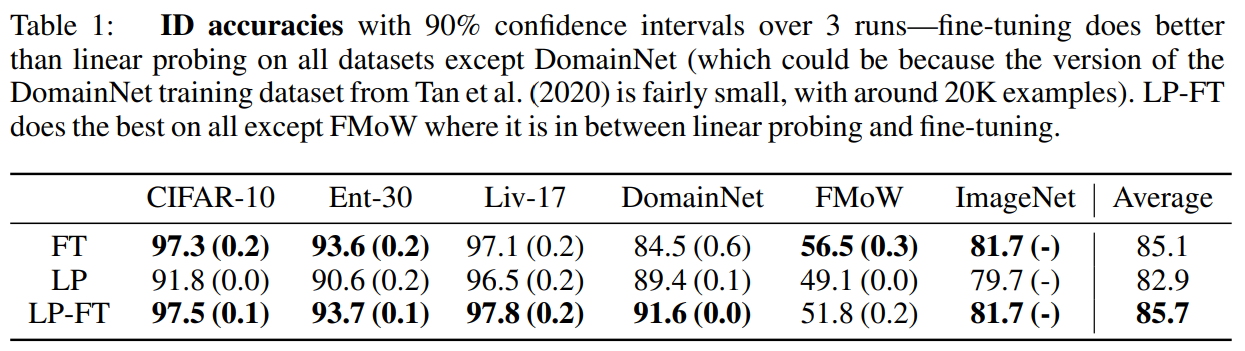
\includegraphics[width=\textwidth]{figures/table-1.png}
    \end{figure}

\end{frame}

\begin{frame}
    \frametitle{Results (2/2)}

    \begin{figure}[htbp]
        \centering
        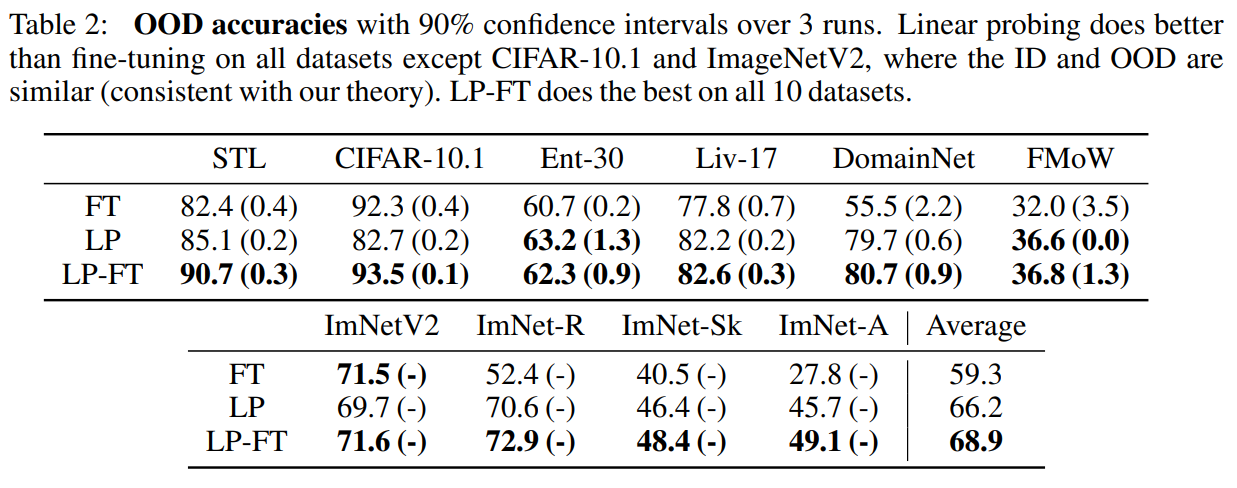
\includegraphics[width=\textwidth]{figures/table-2.png}
    \end{figure}

\end{frame}

\begin{frame}
    \frametitle{Results: Linear Probing Then Fine-Tuning (LP-FT)}

    We find that LP-FT gets the best accuracy ID (average: 85.7\%) and OOD (average: 68.9\%).

    This is true for 5/6 ID and 10/10 OOD datasets---every dataset except FMoW ID, where LP-FT is better than linear probing but worse than fine-tuning.

    Since the ID accuracy on FMoW is low (56.5\%), this could be because the pretrained features are not good.

\end{frame}

\begin{frame}
    \frametitle{Examining the Feature Distortion Theory}

    \begin{itemize}
        \item Early stopping does not mitigate feature distortion.
        \item ID-OOD features get distorted from fine-tuning.
        \item Pretrained features must be good, ID-OOD far apart.
    \end{itemize}

\end{frame}

\begin{frame}
    \frametitle{ID-OOD Features Get Distorted From Fine-Tuning}

    The feature distortion theory predicts that fine-tuning changes features for ID examples more than for OOD examples, which is why fitting a head on ID examples performs poorly OOD.

    To test this, for each example $x$ in Living-17, we took the Euclidean distance of the ResNet-50 features before and after fine-tuning: $\| g_B(x) - g_{B_0}(x) \|_2$.

    As expected, the average distance for ID examples ($0.0188 \pm 0.0001$) is more than for OOD examples ($0.0167 \pm 0.0001$).

    The theory also predicts that LP-FT changes features less than fine-tuning does. As expected, the average distance changed by LP-FT both ID ($0.0011 \pm 0.0001$) and OOD ($0.0009 \pm 0.0001$) is $20\times$ smaller than for fine-tuning.

\end{frame}

\begin{frame}
    \frametitle{Pretrained Features Must Be Good, ID-OOD Far Apart}

    Our theory says that linear probing does better than fine-tuning OOD, but {\color{magenta} only if the OOD and ID data are quite different, and the pretrained features are good}---otherwise fine-tuning can do better OOD by adjusting the feature extractor ID.

\end{frame}

\begin{frame}
    \frametitle{Feature Quality}

    We use a checkpoint of MoCo-v1 that got 10\% worse accuracy (on ImageNet) and compare linear probing and fine-tuning on Living-17.

    With worse features, both methods do worse, but fine-tuning (96\% ID, 71\% OOD) does better than linear probing (92\% ID, 66\% OOD).

\end{frame}

\begin{frame}
    \frametitle{ID $\approx$ OOD}

    We fine-tune/linear probe on CIFAR-10, and test on CIFAR-10.1, a dataset collected using a similar protocol to CIFAR-10.
    
    As expected, fine-tuning (92.3\%) outperforms linear probing OOD (82.7\%).
    
    Even in this case, where we have no tradeoffs, LP-FT does the best (93.5\%).

\end{frame}

\begin{frame}
    \frametitle{Conclusion (1/2)}

    Summary:

    \begin{itemize}
        \item Preserving features might be important for robustness, and simpler approaches like linear probing can improve out-of-distribution (OOD) performance.
        \item This OOD gap between fine-tuning and linear probing grows as the quality of pretrained features improve.
        \item LP-FT can mitigate tradeoffs between ID and OOD accuracy in our context.
    \end{itemize}
    
\end{frame}

\begin{frame}
    \frametitle{Conclusion (2/2)}

    LP-FT could be useful in other situations, for example in CLIP we could initialize the final layer with the zero-shot classifier and then fine-tune the entire model, as done in concurrent work (Wortsman et al., 2021).
    
    In NLP, linear probing is not as good---here we could first prompt-tune (Lester et al., 2021) and then fine-tune the entire model.
    
    LP-FT is just a first step in leveraging the intuition from our theoretical analysis and we hope that this work inspires new methods of leveraging powerful pretrained models.

\end{frame}

\end{document}
